\label{memory}
%%%%%%%%%%%%%%%%%%%%%%%%%%%%%%%%%%%%%%%%%%%%%%%%%%%%%%%%%%%%%%%%%%
%%%%%%%%%%%%%%%%%%%%%%%%%%%%%%%%%%%%%%%%%%%%%%%%%%%%%%%%%%%%%%%%%%

\subsection{Introduction}
Le système d'exploitation développé est exécuté sur une architecture \acrshort{IA-32}
(Intel 32 bits) aussi appelée i386. La mémoire est donc adressée sur 32 bits.
$2^{32}=4Go$, on peut en déduire que la taille totale de la mémoire adressable est
de 4Go dans notre système d'exploitation. Avoir un espace adressable de 4Go ne veut
pas forcément dire que la mémoire physique (\acrshort{ram}) est également de 4Go.
En réalité, la taille de la \acrshort{ram} dépend du \textit{hardware}. Dans notre
cas le matériel est émulé par QEMU. La taille de la mémoire physique de notre \acrshort{os}
dépend de la configuration de l'émulateur. Ces 4Go sont donc virtuels. Lorsqu'une
tache est exécutée, elle est chargée en mémoire et est définie par la paire base
et limite. La base est son adresse physique dans la \acrshort{ram} et la limite
est sa taille. La figure \ref{ex_base_limit} donne un exemple d'adressage de plusieurs
processus \cite{ref42}.

\begin{figure}[!h]
  \centering
  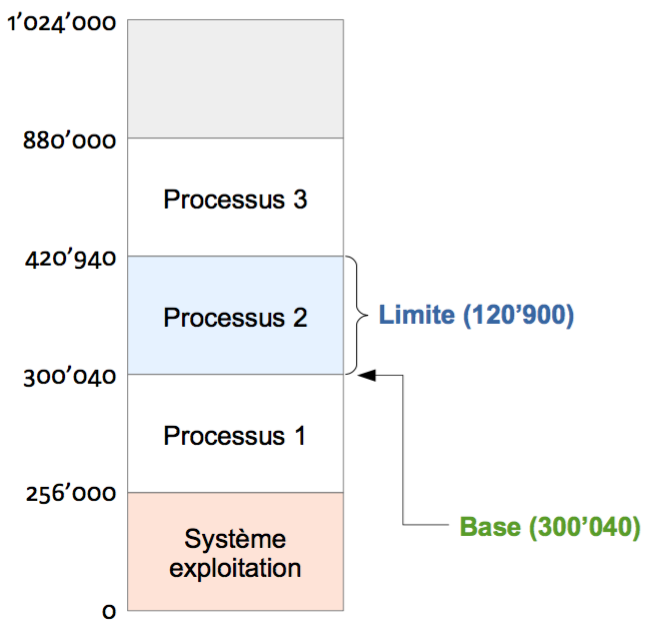
\includegraphics[scale=0.6]{images/ex_base_limit.png}
  \caption{Exemple d'adressage mémoire}
  \label{ex_base_limit}
\end{figure}

Une tache possède son propre espace d'adressage dit virtuel. Pour le processus 2
de la figure \ref{ex_base_limit}, l'adresse 0 est en fait à l'adresse physique
300'040. Il y a donc besoin de translater l'adresse virtuelle en adresse physique.
C'est là qu'entre en jeu le \acrshort{mmu} (\textit{Memory Mangement Unit}). Le \acrshort{mmu}
est un dispositif matériel permettant de faire cette translation d'adresses. A chaque
référencement mémoire, il va convertir l'adresse virtuelle en adresse physique et
regarder si elle ne dépasse pas la limite du processus. Le \acrshort{mmu} permet donc
aussi de protéger la mémoire en empêchant toute référence à une zone extérieure
au processus (voir figure \ref{mmu}) \cite{ref42}.

\begin{figure}[!h]
  \centering
  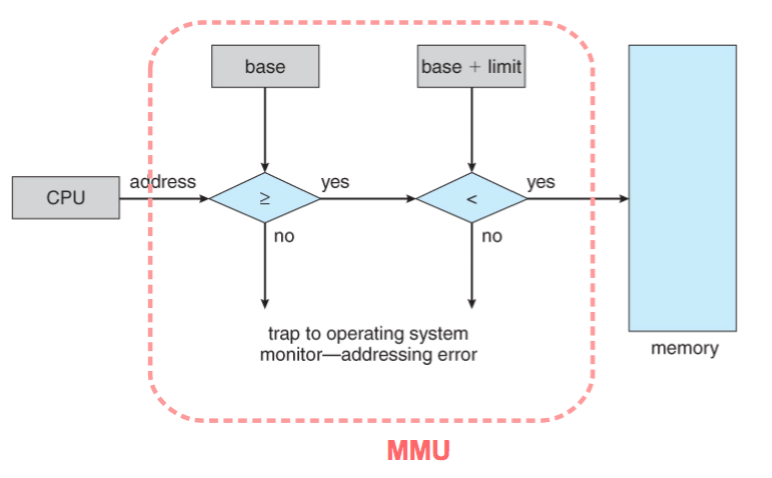
\includegraphics[scale=0.4]{images/mmu.png}
  \caption{Protection mémoire avec un \acrshort{mmu}}
  \label{mmu}
\end{figure}

Pour convertir une adresse virtuelle en adresse physique, le \acrshort{mmu} passe
par plusieurs étapes. Quand le \textit{kernel} veut lire une donnée dans la mémoire,
l'adresse de cette donnée est appelée adresse logique. Le \acrshort{mmu} va commencer
par convertir cette adresse en adresse linéaire. Une deuxième conversion est ensuite
effectuée afin d'obtenir une adresse physique. Le \acrshort{mmu} peut alors renvoyer
la bonne donnée au \textit{kernel}. Toutes ces étapes ne sont pas automatiques,
le \acrshort{mmu} utilise différentes techniques ayant besoin de certaines structures
implémentées par le \textit{kernel}. Ces techniques sont la segmentation et la
pagination.

\begin{figure}[!h]
  \centering
  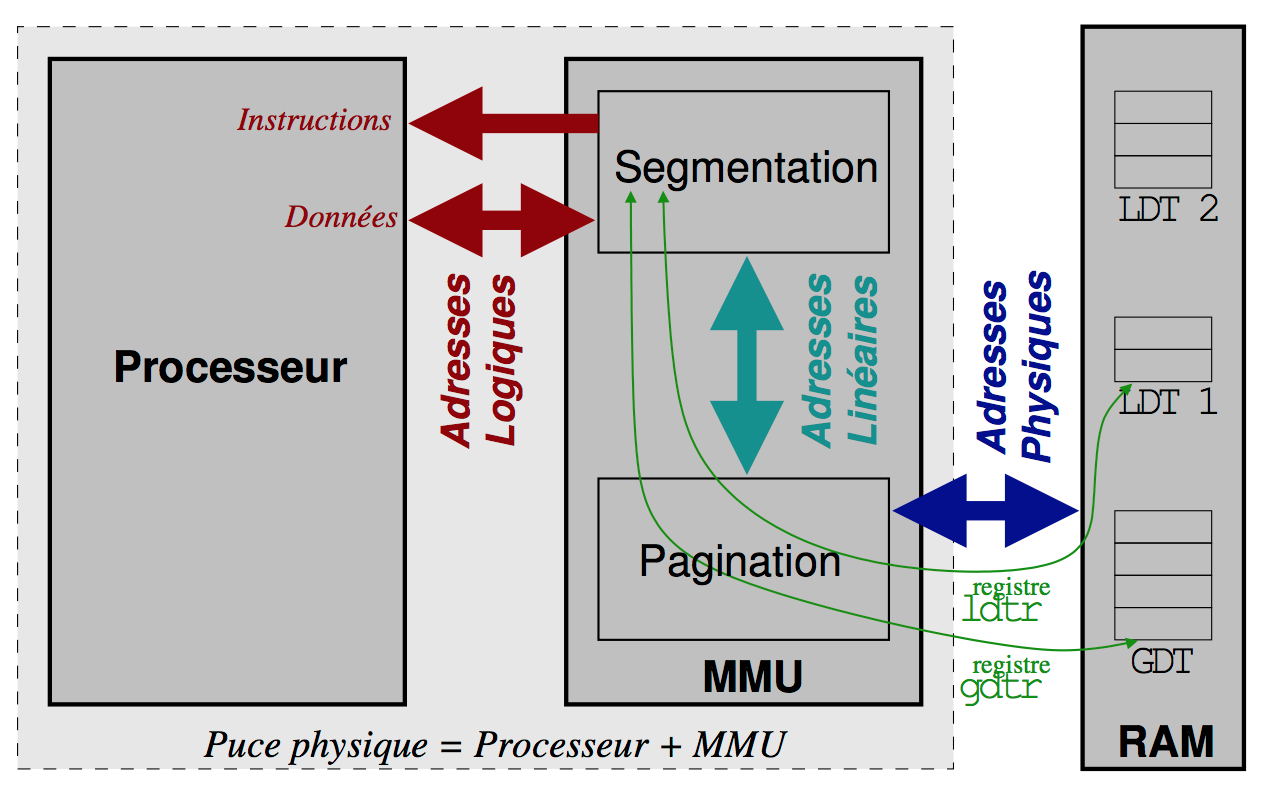
\includegraphics[scale=0.5]{images/addr_translation.png}
  \caption{Translation d'adresse}
  \label{addr_translation}
\end{figure}

La segmentation est une technique permettant de découper la mémoire en segments
de mémoire logique. Une adresse logique est convertie par le \acrshort{mmu} en
adresse linéaire en utilisant une table de descripteurs globale (\acrshort{gdt})
ou locale (\acrshort{ldt}). Si la pagination est activée, l'adresse linéaire est
convertie en adresse physique. Toute cette mécanique est décrite dans la figure
\ref{addr_translation}. A noter que la pagination n'est pas obligatoire et un
\acrshort{os} pourrait s'en passer contrairement à la segmentation qui est
indispensable en mode protégé (32 bits) \cite{ref17}.

%%%%%%%%%%%%%%%%%%%%%%%%%%%%%%%%%%%%%%%%%%%%%%%%%%%%%%%%%%%%%%%%%%
%%%%%%%%%%%%%%%%%%%%%%%%%%%%%%%%%%%%%%%%%%%%%%%%%%%%%%%%%%%%%%%%%%

\subsection{Segmentation}
\subsubsection{Principe général}
Comme expliqué précedemment, la segmentation est un mécanisme divisant l'espace
d'adressage du processeur en espaces d'adressage plus petits appelés des
segments. Un segment peut être utilisé pour contenir le code, les données ou la
pile d'un processus étant exécuté par le processeur. Un segment peut aussi être
utilisé pour contenir des structures de données tel qu'une \acrshort{ldt} ou
un \acrshort{tss} (structure contenant des informations à propos d'une tâche).
Les segments d'un système d'exploitation sont contenus dans l'espace d'adressage
linéaire. Pour lire l'octet d'un segment se trouvant dans l'espace d'adressage
linéaire, le \acrshort{mmu} utilise une adresse logique. L'adresse logique est
composée d'un sélecteur de segment et d'un \textit{offset}. Le sélecteur permet
de trouver le bon segment dans la mémoire linéaire et l'\textit{offset} permet
de trouver l'octet dans ce segment. Dans le cas où la segmentation est utilisée
seule (sans pagination), la mémoire linéaire est \textit{mappée} directement dans
la mémoire physique \cite{ref66}. \\

\begin{figure}[!h]
  \centering
  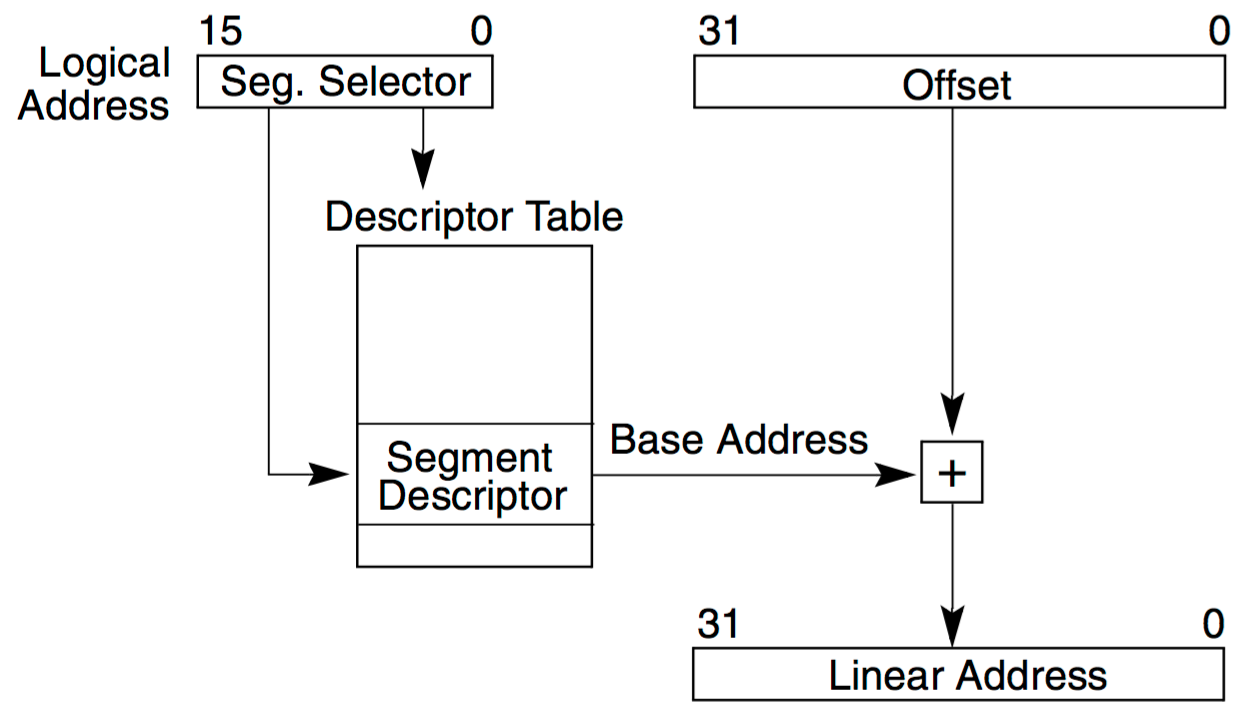
\includegraphics[scale=0.43]{images/logic_addr_conv.png}
  \caption{Conversion d'une adresse logique en adresse linéaire}
  \label{logic_addr_conv}
\end{figure}

La figure \ref{logic_addr_conv} résume la conversion d'adresse logique en
adresse linéaire. On peut remarquer que le sélecteur de segment passe
par une table de descripteurs (\acrshort{gdt} ou \acrshort{ldt}) afin de trouver
le bon segment dans la mémoire linéaire. En effet, un sélecteur a une taille de
16 bits et contient : l'index d'un descripteur dans une table, un bit indiquant si
le descripteur est dans la \acrshort{gdt} ou dans une \acrshort{ldt} et enfin son
niveau de privilège allant de 0 à 3 (figure \ref{seg_sel}) \cite{ref42}.

\begin{figure}[!h]
  \centering
  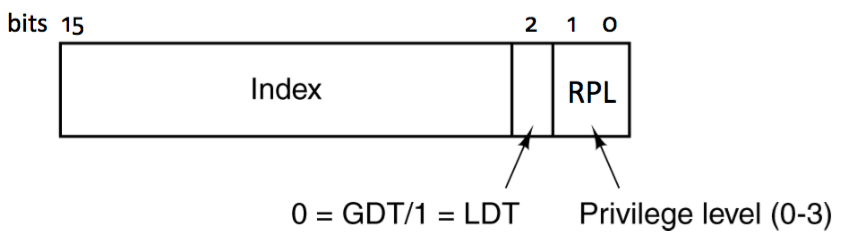
\includegraphics[scale=0.6]{images/seg_sel.png}
  \caption{Structure d'un sélecteur de segment}
  \label{seg_sel}
\end{figure}

La gestion de la segmentation par le \acrshort{cpu} se fait à l'aide de registres
spéciaux nommés registres de segment. Ces registres sont au nombre de six et ont
chacun une taille de 16 bits (même taille qu'un sélecteur de segment) \cite{ref42,ref18}.

\begin{center}
	\scalebox{.8}{
		\begin{tabular}{| C{5cm} | C{5cm} | }
			\hline
			Registre & Segment \\ \hline
			CS & \textit{Code Segment} \\ \hline
			DS & \textit{Data Segment} \\ \hline
			SS & \textit{Stack Segment} \\ \hline
			ES & \textit{Extra Segment} \\ \hline
			FS / GS & \textit{General Purpose Segments} \\ \hline
		\end{tabular}
	}
    \captionof{table}{Registres de segment}
    \label{table_seg_reg}
\end{center}

En mode protégé (32 bits), ces registres doivent pointer sur des descripteurs
de segment de la \acrshort{gdt}. Au minimum les trois premiers registres décrits
doivent être utilisés en mode protégé (CS, DS, et SS). Les opérations adressant
le code (décodage des instructons en mémoire, sauts, etc...) référencent le descripteur
de segment sur lequel pointe le registre CS. Les opérations adressant les données
(adressage de variables ou d'adresses mémoires) référencent le descripteur de segment
sur lequel pointe le registre DS. Les opérations adressant la pile (\mintinline{text}{push}
et \mintinline{text}{pop}) référencent le descripteur de segment sur lequel pointe
le registre SS. Ces registres pointent sur des descripteurs de segments par l'intermédiaire
de sélecteurs de segment. \\

%%%%%%%%%%%%%%%%%%%%%%%%%%%%%%%%%%%%%%%%%%%%%%%%%%%%%%%%%%%%%%%%%%

\subsubsection{\acrshort{gdt} et \acrshort{ldt}}
\label{gdt_ldt}
Nous avons pu voir que pour translater une adresse logique, des sélecteurs de
segment sont utilisés. Ces sélecteurs pointent sur des entrées dans des tables
de descripteurs. La \acrshort{gdt} et la \acrshort{ldt} sont deux types de table 
de descripteurs différents. La \acrshort{gdt} est unique il ne peut y en avoir
qu'une seule dans le système. Elle contient toutes les données utilisables en mode
superviseur (\textit{ring} 0 ou niveau de privilège 0). Une \acrshort{ldt} est
contenue dans la \acrshort{gdt}. Elle peut être utilisée pour contenir le code
et les données d'une tâche utilisateur par exemple. Dans le cas où plusieurs tâches
sont exécutées en même temps, une \acrshort{ldt} peut être créée par tâche ce qui
permet en plus d'isoler le code de chaque processus. Une table de descripteurs
est composée, comme son nom l'indique, de descripteurs. Chaque descripteur décrit
une zone mémoire qui est définie par sa base (son adresse physique), sa limite (sa taille)
et un niveau de privilèges (allant de 0 à 3, le niveau 0 ayant le plus de privilèges
et le niveau 3 le moins). Ci dessous, la figure \ref{gdt} montre un exemple d'une
\acrshort{gdt} \cite{ref42}. Etant donné que les descripteurs de la \acrshort{gdt}
ont la même structure que les descripteurs de la \acrshort{ldt} nous allons nous
concentrer sur la \acrshort{gdt}. De plus, aucune \acrshort{ldt} n'est utilisé dans
la version actuelle de l'\acrshort{os}. \\

\begin{figure}[!h]
  \centering
  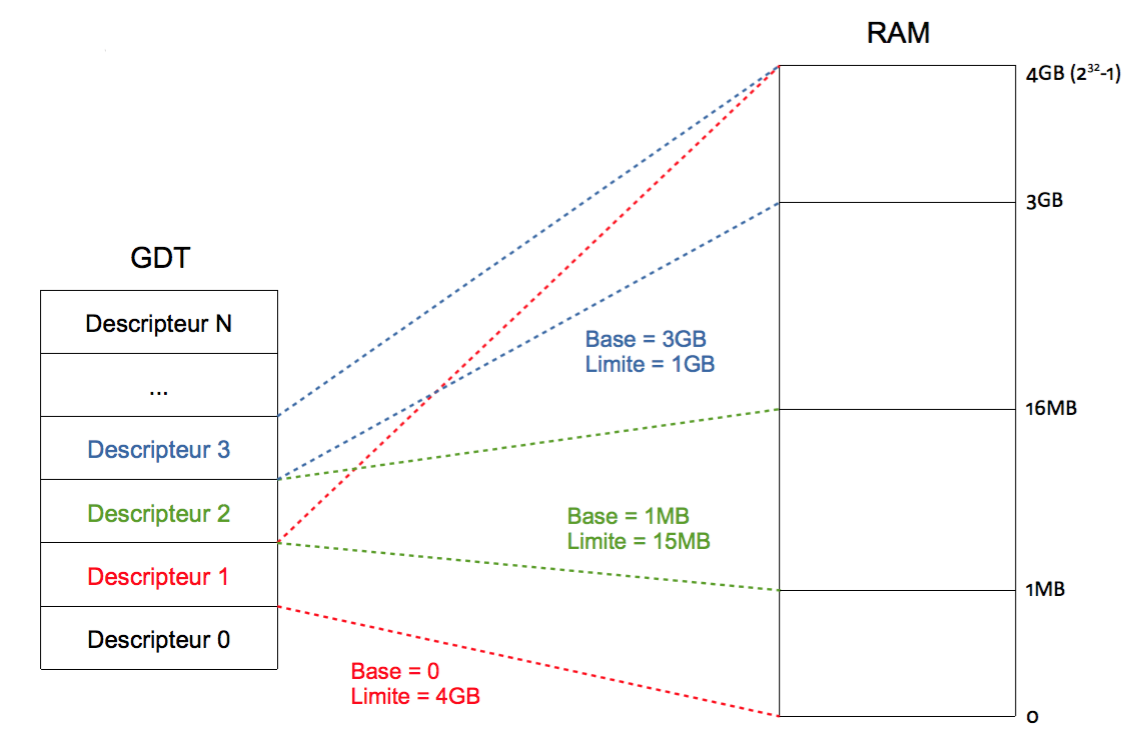
\includegraphics[scale=0.75]{images/gdt.png}
  \caption{Exemple d'une \acrshort{gdt}}
  \label{gdt}
\end{figure}

La \acrshort{gdt} est contenue en mémoire. Cette dernière doit être initialisée
par le \textit{kernel} avant d'être chargée et utilisée par le \acrshort{mmu}.
Pour initialiser la \acrshort{gdt} il faut construire ses entrées. Chaque entrée
(ou descripteur) de la table de descripteurs est sur 64 bits et décrit une zone
mémoire. L'adresse de cette zone mémoire est sur 32 bits et sa taille est sur 20
bits. Les bits restant sont des bits de contrôle pour l'accès aux données par
exemple (niveau de privilèges, droit d'écriture/lecture, ...). Voir la figure
\ref{gdt_entry} pour plus de détails \cite{ref42,ref14}. \newpage

\begin{figure}[!h]
  \centering
  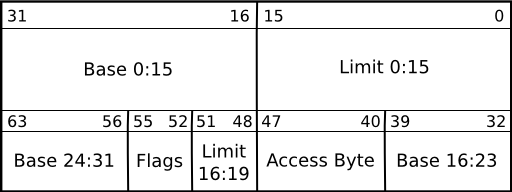
\includegraphics[scale=0.75]{images/gdt_entry.png}
  \caption{Structure d'une entrée dans la \acrshort{gdt}}
  \label{gdt_entry}
\end{figure}

L'\acrshort{os} développé a un adressage segmenté de type \textit{flat}, c'est-à-dire
que toute la mémoire est accédée de manière linéaire. Ce modèle de segmentation
est le plus simple puisqu'il permet d'ignorer le mécanisme de segmentation car
l'intégralité de la zone mémoire devient alors disponible. Dans un modèle de type \textit{flat},
les segments de code et de données se chevauchent sur l'intégralité de la mémoire
disponible. Ceci se fait en initialisant trois descripteurs dans la \acrshort{gdt} :
un descripteur nul à l'index 0 (obligatoire dans tous les modèles de segmentation),
un segment de code couvrant toute la mémoire et un segment de données couvrant
aussi toute la mémoire. Les segments de code et de données adressent ainsi les mêmes
zones mémoire. On verra par la suite que d'autres entrées ont été aujoutées à la
\acrshort{gdt} pour la gestion des tâches. \\

\begin{figure}[!h]
  \centering
  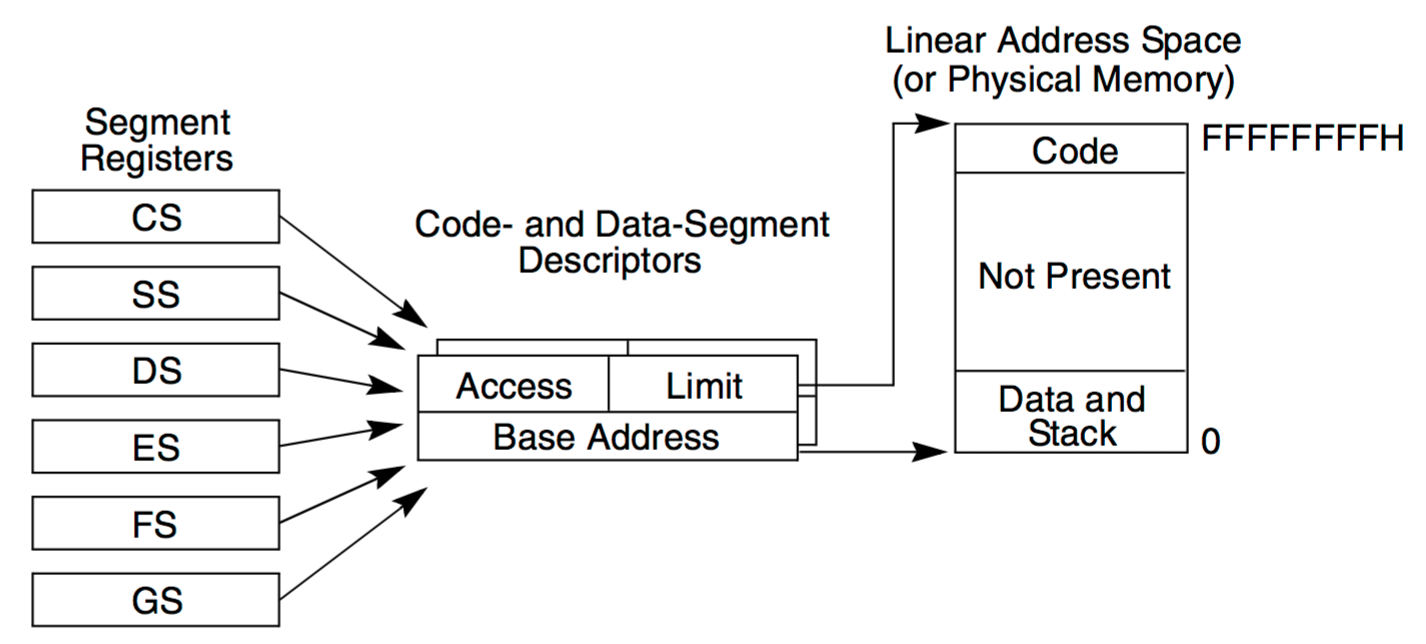
\includegraphics[scale=0.6]{images/flat.png}
  \caption{Modèle de segmentation de type \textit{flat}}
  \label{flat}
\end{figure}

Pour obtenir un  segment sur toute la mémoire disponible, il faut mettre le bit
de granularité à 1 pour avoir une limite en blocs de 4Ko. Ensuite, la limite doit
être mise à la valeur 0xFFFFF ce qui donne une limite réelle de 0x100000 $\times$
0x1000 soit 4Go. Le niveau de privilège doit être laissé à 0 (\textit{ring} 0)
si on veut créer un segment pour le \textit{kernel} ou bien être mis à 3 (\textit{ring}
3) si on veut créer un segment pour le mode utilisateur. Ci-dessous un exemple de
code permettant de construire un segment de code et un segment de données. \newpage

\begin{code}
\begin{minted}[fontsize=\footnotesize,tabsize=4,frame=single,linenos]{rust}
fn new(base: u32, limit: u32, type: u8, s: u8, d: u8, g: u8, dpl: u8) -> GdtEntry;

pub fn make_code_segment(base: u32, limit: u32, dpl: u8) -> GdtEntry {
    GdtEntry::new(base, limit, 0xB, 0x1, 0x1, 0x1, dpl)
}

pub fn make_data_segment(base: u32, limit: u32, dpl: u8) -> GdtEntry {
    GdtEntry::new(base, limit, 0x3, 0x1, 0x1, 0x1, dpl)
}
\end{minted}
\caption{Constructeurs d'une entrée dans la \acrshort{gdt}}
\label{lst:mem:gdt:constructors}
\end{code} \bigbreak

Ici, \mintinline{rust}{new} est le prototype d'une méthode pour une structure 64
bits représentant une entrée dans la \acrshort{gdt}. Le bit \mintinline{rust}{s}
est mis à 1 car on construit des segments de code et de données \cite{ref66}.
Le bit \mintinline{rust}{d} est mis à 1 car on veut un segment de 32 bits. Le bit
\mintinline{rust}{g} est mis à 1 pour avoir une granularité de 4Ko. L'octet 0xB
correspond au type $CODE\_EXEC\_READ$ et 0x3 correspond au type $DATA\_READ\_WRITE$
\cite{ref42}. Une fois la \acrshort{gdt} construite, il faut dans un premier temps
utiliser l'instruction \mintinline{text}{lgdt} pour la charger dans le registre
GDTR. Ce registre est utilisé par le processeur pour faire le lien entre le \acrshort{mmu}
et la \acrshort{gdt} créée \cite{ref66}. L'adresse du descripteur de la \acrshort{gdt}
doit donc être donnée en argument à l'instruction \mintinline{text}{lgdt}. Le
descripteur de \acrshort{gdt} est défini par la structure 48-bits décrite dans
la figure suivante \cite{ref14}.

\begin{figure}[!h]
  \centering
  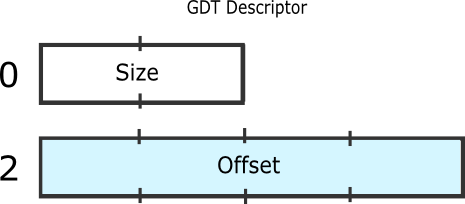
\includegraphics[scale=0.5]{images/gdt_descriptor.png}
  \caption{Descripteur de \acrshort{gdt}}
  \label{gdt_descriptor}
\end{figure}

Dans un descripteur de \acrshort{gdt}, \textit{Size} est la limite sur 16 bits
(c'est à dire la taille de la \acrshort{gdt} - 1) et \textit{Offset} est l'adresse
physique de la \acrshort{gdt} sur 32 bits. Dans le cas de notre \acrshort{os},
la \acrshort{gdt} est déclarée statiquement dans le \textit{kernel}. L'adresse
de cette variable statique est utilisée pour construire un descripteur qui sera
chargé dans le registre GTDR. Après avoir chargé la \acrshort{gdt} avec l'instruction
\mintinline{text}{lgdt}, il faut faire pointer les registres de segment sur les
segments de la table de descripteurs à l'aide de sélecteurs. Pour rappel, un sélecteur
est sur 16 bits et contient l'index d'un segment dans la \acrshort{gdt} précedemment
chargée. Pour récupérer l'index d'un segment dans la \acrshort{gdt} à partir de
l'index de son descripteur, il faut faire un décalage à gauche de 3 bits
(voir figure \ref{seg_sel}). Prenons un descripteur se situant à l'index 2 de
la \acrshort{gdt}. Si on veut initialiser le segment de code (registre CS) avec
ce descripteur, il faut mettre la valeur 16 dans le registre CS ($2 << 3 = 16$).
Dans le cas où l'on veut définir ce segment avec un autre niveau de privilèges
ou bien pour une \acrshort{ldt}, il suffit de mettre les bons bits à 1 après avoir
fait le décalage.

\newpage
%%%%%%%%%%%%%%%%%%%%%%%%%%%%%%%%%%%%%%%%%%%%%%%%%%%%%%%%%%%%%%%%%%
%%%%%%%%%%%%%%%%%%%%%%%%%%%%%%%%%%%%%%%%%%%%%%%%%%%%%%%%%%%%%%%%%%

\subsection{Pagination}
\subsubsection{Principe général}
La pagination est une autre technique de gestion de mémoire qui diffère de la
segmentation. Alors que la segmentation permet d'allouer des morceaux de mémoire
de taille variable, la pagination divise la mémoire en blocs de taille fixe appelés
pages (de 4Ko, 2Mo ou 4Mo). De plus, la segmentation est obligatoire dans une
architecture i386 alors que la pagination ne l'est pas \cite{ref16}. Quand une tâche
fait référence à une adresse logique en mémoire, cette adresse est convertie en
adresse linéaire grâce au mécanisme de segmentation. C'est le mécanisme de
pagination qui permet de translater cette adresse linéaire en adresse physique
(comme vu précedemment dans la partie sur la segmentation). Quand la
pagination est activée, l'adresse linéaire est divisée en deux parties lorsque
des pages de 4Mo sont utilisées et en trois parties lorsque des pages de 4Ko
sont utilisées. Le \textit{kernel} développé utilise des pages de 4Ko, une adresse
linéaire est donc sous la forme suivante :

\begin{itemize}[label=\textbullet]
	\item 10 bits pour le \textit{directory index}
	\item 10 bits pour le \textit{page index}
    \item 12 bits pour l'\textit{offset}
\end{itemize}

On dit que cette pagination est une pagination à trois niveaux. En général, une
pagination à trois niveaux est utilisée mais il peut exister des systèmes utilisant
plus ou moins de niveaux. Le système d'exploitation doit créer un répertoire de pages
(\textit{Page Directory}) et au moins une table des pages (\textit{Page Table}) pour
chaque tâche. Les répertoires et les tables des pages ont la taille d'une page et sont
composés d'entrées sur 32 bits (4 octets). Une entrée dans un répertoire permet
d'adresser une table de pages et une entrée dans une table permet d'adresser une page.
Dans notre cas, un répertoire permet donc d'adresser 1024 tables et une table
1024 pages ce qui permet bien d'adresser au total 4Go ($1024 \times 1024 \times 4096$).
Une entrée est sur 32 bits mais seulement les 20 bits de poids fort sont utilisés
pour l'adressage car les adresses sont alignées avec 4096 ce qui laisse les 12 bits
de poids faible pour la configuration \cite{ref21}.

\begin{figure}[!h]
  \centering
  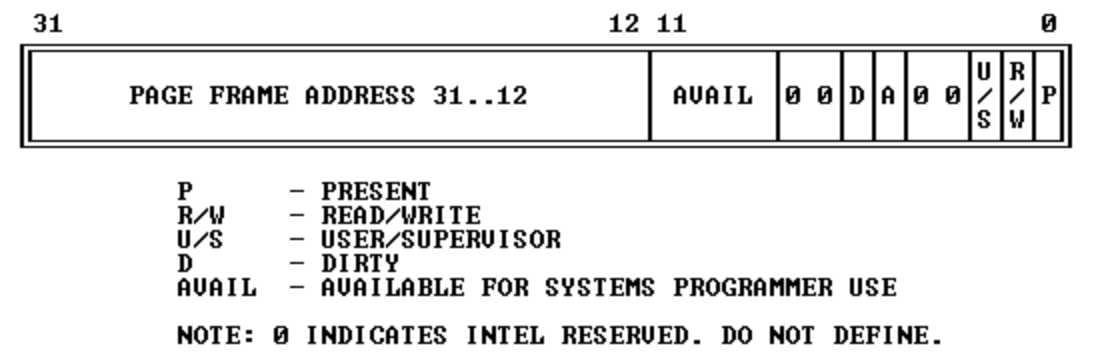
\includegraphics[scale=0.6]{images/page_entry.png}
  \caption{Structure d'une \textit{Page Entry}}
  \label{page_entry}
\end{figure}

Quand une adresse linéaire est lue, le \textit{directory index} permet
de lire la bonne entrée dans le \textit{Page Directory}. Il faut ensuite utiliser
le \textit{page index} pour récupérer la bonne entrée dans la table des pages.
De la même manière que l'entrée dans le répertoire de pages pointait sur une table
des pages, l'entrée dans une table des pages pointe sur une \textit{Page Frame}.
Cette page contient finalement la donnée pointée par l'adresse linéaire, il faut
utiliser l'\textit{offset} pour trouver cette donnée dans la page. La figure \ref{paging3}
résume bien ce mécanisme \cite{ref66}. A noter que le \textit{Page Directory} est
pointé par le registre CR3. A chaque fois qu'un changement de tâche a lieu, le
registre CR3 doit être mis à jour avec le \textit{Page Directory} de la nouvelle
tâche \cite{ref15}.

\begin{figure}[!h]
  \centering
  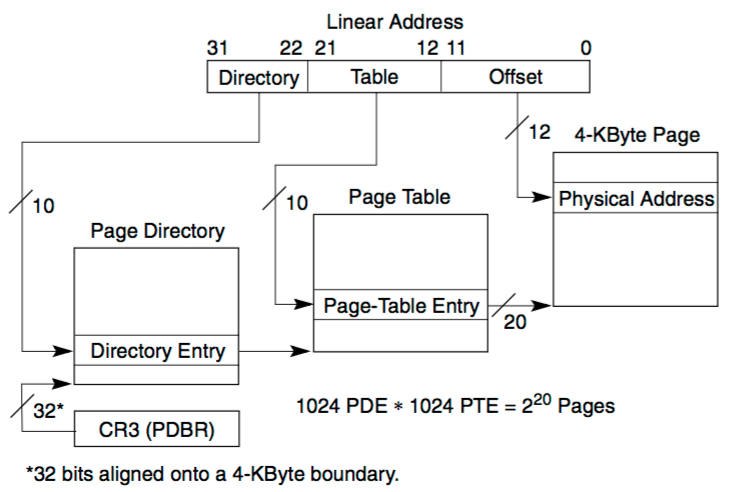
\includegraphics[scale=0.85]{images/paging3.png}
  \caption{Exemple de pagination à 3 niveaux}
  \label{paging3}
\end{figure}

%%%%%%%%%%%%%%%%%%%%%%%%%%%%%%%%%%%%%%%%%%%%%%%%%%%%%%%%%%%%%%%%%%

\subsubsection{Activation de la pagination}
\label{activate_paging}
Pour initialiser la pagination sur architecture x86, il faut d'abord construire
un répertoire de pages valide contenant les entrées vers les pages du \textit{kernel}.
Il est obligatoire de commencer par cela car si la pagination est activée et que
le \textit{kernel} n'est pas \textit{mappé} dans le répertoire chargé, une exception
sera levée (\textit{Page Fault}). Par soucis de simplicité pour la suite du développement
de l'\acrshort{os}, le \textit{kernel} va être déplacé au dernier Go de la \acrshort{ram}.
Grace à la pagination, ceci peut se faire assez simplement, il suffit de compléter
le répertoire de pages ainsi que ses tables de pages correctement. Pour rappel,
le \textit{kernel} commence à l'adresse 0x100000 (1Mo) mais il faut aussi rendre
accessible le premier mégaoctet de \acrshort{ram}. Il faut donc déplacer les adresses physiques
allant de 0x0 à la fin du kernel (qui n'est pas fixe). Dans un premier temps, le
\textit{linker} doit être modifié de cette manière :

\begin{code}
\begin{minted}[fontsize=\footnotesize,linenos,frame=single,tabsize=4]{c}
SECTIONS {
    /* Low memory Kernel */
    . = 0x00100000;
    .boot ALIGN(4) :        { *(.multiboot) }
    .low_text ALIGN (4K) :  { *(.low_text) }
    .low_data ALIGN (4K) :  { *(.low_data) }
    .low_bss ALIGN (4K) :   { *(.low_bss) }
    /* Higher-half Kernel */
    . += 0xC0000000;
    .stack ALIGN(4) : AT(ADDR(.stack) - 0xC0000000)     { *(.stack) }
    .text ALIGN(4K) : AT(ADDR(.text) - 0xC0000000)      { *(.text*) }
    .rodata ALIGN(4K) : AT(ADDR(.rodata) - 0xC0000000)  { *(.rodata*) }
    .data ALIGN(4K) : AT(ADDR(.data) - 0xC0000000)      { *(.data*) }
    .bss ALIGN(4K) : AT(ADDR(.bss) - 0xC0000000)        { *(COMMON) *(.bss*) }
}
\end{minted}
\caption{\textit{Linker script} du \textit{higher-half kernel}}
\label{lst:mem:paging:linker}
\end{code} \bigbreak

Ici, le \textit{kernel} est divisé en deux parties. La première est celle qui va
être appelée au démarrage du système et qui va initialiser la pagination. Une fois
la pagination active, le \textit{kernel} va continuer son exécution dans la deuxième
partie qui est située dans le dernier gigaoctet de \acrshort{ram}. Nous sommes obligés de
démarrer le \textit{kernel} au début de la mémoire physique car toutes les adresses
sont virtuelles. Nous utilisons QEMU pour émuler le matériel. La taille de la \acrshort{ram}
dépend de la configuration de celui-ci. Il n'existe donc peut-être pas d'adresse
physique située à 3Go dans la \acrshort{ram} et il pourrait donc être impossible de
démarrer le système à cette adresse (ce qui est notre cas). Regardons plus en détail de quelle
manière la première partie du \textit{kernel} initialise la pagination. Comme expliqué,
un répertoire de pages initial doit être construit. Etant donné que nous allons
exécuter du code dans le premier gigaoctet et également dans le dernier, le \textit{kernel}
doit être \textit{mappé} dans ces deux zones mémoire en même temps. La première
partie va être adressée linéairement, ce qui veut dire que l'adresse physique
0x0 correspondra à l'adresse virtuelle 0x0 et ainsi de suite jusqu'à la fin du
\textit{kernel}. Cet adressage donne le répertoire de pages schématisé dans la figure
\ref{low_kern_pd}.

\begin{figure}[!h]
  \centering
  \includegraphics[scale=0.65]{images/low_kern_pd.png}
  \caption{Répertoire de pages adressant le \textit{kernel} au début de la \acrshort{ram}}
  \label{low_kern_pd}
\end{figure}

On peut voir ici que la première entrée du répertoire de pages pointe sur une
table de pages adressant le début de la \acrshort{ram}. Chaque entrée est incrémentée
de 4096 (0x1000 en hexadécimal) car une page fait 4096 octets. De plus, les deux
premiers bits de poids faible de chaque page sont à 1 pour indiquer que la page est
active et que l'on peut écrire et lire dedans (voir figure \ref{page_entry}). L'entrée
dans le répertoire de pages correspondant au dernier gigaoctet (soit 0xC0000000 en hexadécimal)
doit pointer sur une table des pages identique. Pour trouver une entrée dans le
répertoire de pages depuis une adresse il faut faire un décalage à droite de 22
bits sur cette adresse (ce qui est équivalent à diviser par 4096, soit la taille
d'une page, puis de nouveau diviser par 1024, soit le nombre de pages adressées par
une table). Ici, 0xC0000000 $>>$ 22 = 0x300 (768 en décimal). Il faut donc faire
pointer l'entrée 768 du répertoire de pages à une table des pages identique à
celle pointée par l'entrée 0 ce qui donne finalement le répertoire suivant.

\begin{figure}[!h]
  \centering
  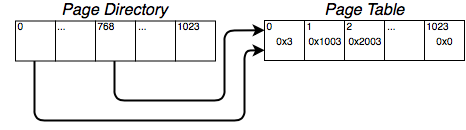
\includegraphics[scale=0.65]{images/high_kern_pd.png}
  \caption{Répertoire de pages adressant le \textit{kernel} à la fin de la \acrshort{ram}}
  \label{high_kern_pd}
\end{figure}

Une fois le répertoire de pages initialisé de cette manière, il ne reste plus
qu'à faire pointer le registre CR3 dessus et activer la pagination en mettant
le bit 31 du registre CR0 à 1. Le pointeur d'instruction peut ensuite sauter à
la partie haute de la \acrshort{ram} où nous avons déplacé le \textit{kernel}. A partir de là,
tout le code qui sera exécuté sera dans le dernier Go de \acrshort{ram}, il n'y
a donc plus besoin de faire pointer la première entrée du répertoire de pages
sur le table des pages du \textit{kernel} ce qui peut être fait en écrivant 0
dans cette entrée. Le code rust peut finalement être appelé avec la pagination
active.

%%%%%%%%%%%%%%%%%%%%%%%%%%%%%%%%%%%%%%%%%%%%%%%%%%%%%%%%%%%%%%%%%%
%%%%%%%%%%%%%%%%%%%%%%%%%%%%%%%%%%%%%%%%%%%%%%%%%%%%%%%%%%%%%%%%%%

\subsection{Allocation dynamique en mode \textit{kernel}}
\label{alloc_kernel}
Le dernier élément de gestion mémoire implémenté dans RustOS est l'allocation de
mémoire dynamique. L'allocation dynamique consiste à réserver des blocs de mémoire
pendant l'exécution du \textit{kernel} ou d'un programme utilisateur. Jusqu'à
maintenant, toutes les structures utilisées était déclarées statiquement, se retrouvant
donc dans la zone mémoire du \textit{kernel}, plus précisément dans le segment
bss (voir \ref{linking}). Déclarer des variables statiquement est pratique mais fait
augmenter la taille du \textit{kernel} ce qui n'est pas une solution viable
pour allouer de plus grandes régions mémoire. Par exemple du code utilisateur
pouvant faire plusieurs kilooctets. Pour implémenter l'allocation de mémoire
dynamique, il faut dans un premier temps définir quelle zone mémoire peut être
utilisée dans ce but. Actuellement, la totalité du code et des données est contenu
dans le \textit{kernel}. Des zones mémoires peuvent donc commencer à être allouées
à la fin de ce dernier. Le \textit{linker} a été légèrement modifié afin d'obtenir
l'adresse de la fin du \textit{kernel}. Ceci peut se faire en ajoutant une expression
au \textit{linker} et en la rendant accessible depuis le code assembleur. \\

\begin{code}
\begin{minted}[fontsize=\footnotesize,linenos,frame=single,tabsize=4]{c}
. += 0xC0000000;
...
kernel_end = .;
\end{minted}
\caption{Modification apportée au \textit{linker}}
\label{lst:mem:alloc:linker}
\end{code} \bigbreak

\begin{code}
\begin{minted}[fontsize=\footnotesize,linenos,frame=single,tabsize=4]{text}
extern kernel_end
get_kernel_end:
    mov eax, kernel_end
    ret
\end{minted}
\caption{Code assembleur rendant accessible l'expression \mintinline{c}{kernel_end}}
\label{lst:mem:alloc:kernel_end}
\end{code} \bigbreak

A partir de là, on peut définir la zone d'allocation mémoire aussi appelée tas
(ou \textit{heap} en anglais). Dans notre \acrshort{os}, le tas commence à la
fin du \textit{kernel} alignée avec la taille d'une page (4096 octets). Ce choix
a été fait car le \textit{kernel} n'aura besoin d'allouer que des nouvelles
pages. La fin du tas dépend de la fin de la mémoire physique qui dépend de la
configuration de QEMU. Quand le \textit{kernel} aura besoin d'allouer une nouvelle
page, il ira chercher le prochain bloc libre dans le tas situé entre la fin
du \textit{kernel} et la fin de la mémoire physique. La recherche de bloc libre
se complexifie rapidement si des blocs sont libérés. De nombreuses méthodes sont
possibles pour la recherche de blocs libres et la gestion des blocs libérés. Le
\textit{kernel} développé utilise une liste doublement chaînée pour gérer la
mémoire dynamique. Chaque bloc mémoire alloué est précédé d'un entête contenant
l'adresse du bloc précédent sur 32 bits, l'adresse du bloc suivant sur 32 bits,
sa taille en octets sur 32 bits et un booléen indiquant si le bloc est libre ou
non sur 8 bits. De plus, l'entête est aligné sur 16 octets.

\begin{figure}[!h]
  \centering
  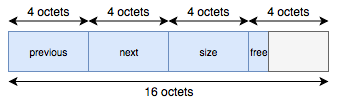
\includegraphics[scale=0.7]{images/heap_header.png}
  \caption{Entête d'un bloc de mémoire dans le tas}
  \label{heap_header}
\end{figure}

Le tas ainsi construit, avec chaque entête lié à ses voisins par des pointeurs,
permet de rechercher aisément un bloc libre. Un nouvel entête est créé quand le
dernier bloc de la liste chaînée est alloué. Un algorithme a aussi été implémenter
pour la gestion de mémoire libérée. Si un bloc est libéré au milieu de blocs
alloués ce bloc est simplement marqué comme libre (en utilisant le booléen \textit{free}
de l'entête). Si deux blocs libres sont contiguës, ils sont fusionnés pour n'en
former qu'un seul. Dans le \textit{kernel}, la fonction pour l'allocation est
\mintinline{rust}{kmalloc} et la fonction pour la libération est \mintinline{rust}{kfree}.
La fonction \mintinline{rust}{kmalloc} va allouer de nouvelles pages et tables
de pages automatiquement s'il y a besoin (voir figure \ref{kmalloc}).
De la même manière, la fonction \mintinline{rust}{kfree} va libérer les pages et
les tables de pages automatiquement. Ces deux fonctions permettent donc beaucoup
d'abstraction au niveau de la pagination mais aussi de l'allocation car l'utilisation
des entêtes est complètement transparente. La fonction \mintinline{rust}{kmalloc}
va simplement renvoyer une adresse sur 32 bits et \mintinline{rust}{kfree} prend
comme argument cette adresse pour libérer la mémoire.

\begin{figure}[!h]
  \centering
  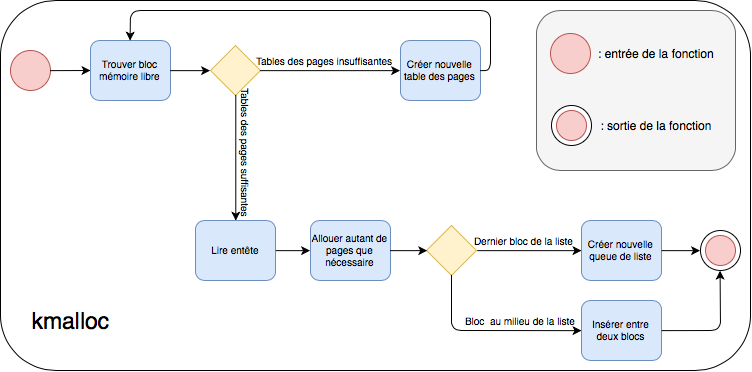
\includegraphics[scale=0.6]{images/kmalloc.png}
  \caption{Algorithme utilisé pour l'allocation dynamique dans le \textit{kernel}}
  \label{kmalloc}
\end{figure}

Voyons maintenant un exemple d'allocation et de libération mémoire utilisant les
deux algorithmes décrits ci-dessus. Dans cet exemple, nous allons allouer plusieurs
blocs mémoire puis les libérer afin de voir plus en détail le comportement
de ces fonctions. Nous allons supposer que la fin du \textit{kernel} se situe
à l'adresse 0x3FC000 et que la fin de la \acrshort{ram} se situe à l'adresse
0x1000000. A l'initialisation du \textit{kernel}, un premier entête est créé au
début de la zone d'allocation dynamique. Ce premier entête est donc situé à
l'adresse 0x3FC000 et a pour taille 0x1000000 $-$ 0x3FC000 $=$ 0xC04000. C'est cette
information qui permet de trouver la première entrée de la liste et par la suite
de la parcourir.

\begin{figure}[!h]
  \centering
  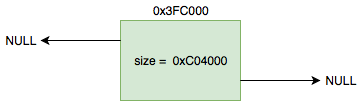
\includegraphics[scale=0.7]{images/alloc0.png}
  \caption{Etat initial de la chaîne d'entêtes}
  \label{alloc0}
\end{figure}

Maintenant, si le \textit{kernel} a besoin d'allouer une nouvelle page, la fonction
\mintinline{rust}{kmalloc} va être appelée et va parcourir les blocs libres. Dans ce cas précis,
l'intégralité du tas est disponible donc la fonction va simplement créer un nouveau
bloc. Dans la figure \ref{alloc1}, les blocs libres sont en vert et les blocs alloués
sont en rouge. A noter que les blocs alloués sont alignés avec la taille d'une
page (4096Ko ou 0x1000 en hexadécimal). Etant donné qu'il faut compter l'entête
de 16 octets, il faudra toujours allouer une page de plus.

\begin{figure}[!h]
  \centering
  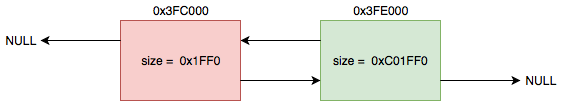
\includegraphics[scale=0.6]{images/alloc1.png}
  \caption{Allocation d'une page}
  \label{alloc1}
\end{figure}

Si le \textit{kernel} a de nouveau besoin d'une page, on va se retrouver dans la
situation où il n'y a plus assez de place dans la table des pages. Pour rappel,
une table des pages a une taille de 4Mo (0x400000 en hexadécimal). Comme expliqué
dans la figure \ref{kmalloc}, la fonction d'allocation va se charger toute seule
de créer une nouvelle table des pages et de l'ajouter au répertoire de pages.
La page demandée par le \textit{kernel} sera ensuite allouée. On obtient donc
la liste de la figure \ref{alloc2}, avec deux blocs alloués au lieu d'un seul.
Le bloc à l'adresse 0x3FE000 contient alors la table des pages sur laquelle pointe
la deuxième entrée du répertoire des pages. La page demandée par le \textit{kernel}
sera finalement à l'adresse 0x400000.

\begin{figure}[!h]
  \centering
  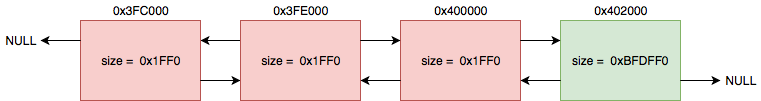
\includegraphics[scale=0.6]{images/alloc2.png}
  \caption{Allocation d'une page et d'une table des pages}
  \label{alloc2}
\end{figure}

Libérer la page à l'adresse 0x400000 aura pour conséquence de libérer également
la table des pages nouvellement créée (la fonction \mintinline{rust}{kfree} libère
automatiquement les tables des pages vides). On se retrouvera alors avec le même
schéma que dans la figure \ref{alloc1} car les blocs aux adresses 0x3FE000 et
0x400000 seront fusionnés au reste de la mémoire libre.